\chapter{Montée en compétences : programmation d'un programme simple}

\paragraph{}Afin d'apprendre à coder en C\# avec WPF, nous avons décidé de commencer par un projet bien plus modeste : le développement d'un jeu de Memory. Il s'agit d'apprendre à coder en C\# avec WPF (et donc à utiliser XAML, comme expliqué au prochain paragraphe), mais aussi de se familiariser avec l'IDE utilisé. Nous avons choisi pour cela Microsoft Visual Studio : le langage C\# a été créé pour être utilisé avec cet IDE, il permet de générer le code XAML à partir d'une interface graphique, possède des outils de déboguage très puissants et une licence est fournie aux élèves de Supélec. Comme gestionnaire de versions, nous utilisons Git.

\begin{figure}[h]
	\begin{minipage}[t]{0.5\textwidth}
		\centering
		
\includegraphics[height=1cm, width=\textwidth, keepaspectratio=true]{logoVS.png}		
	\end{minipage}
	\begin{minipage}[t]{0.5\textwidth}
		\centering
		
\includegraphics[height=1cm, width=\textwidth, keepaspectratio=true]{logoGit.png}		
	\end{minipage}
	\caption{Les logos de Visual Studio 2017 (gauche) et de Git (droite).}
	\label{fig:logos}
\end{figure}


\section{La dualité C\#/XAML}

\paragraph{}Lorsqu'un programme graphique est créé en utilisant WPF, deux langages sont utilisés. Les éléments graphiques (fenêtre, boutons, images, etc...) sont codés en XAML. Il s'agit d'un langage descriptif dérivé du XML. Il nous permet de décrire les attributs de chaque élément : par exemple, la fenêtre a un nom (utilisé pour l'appeler dans le code), un titre, une taille, une position, etc... Elle possède aussi des \enquote{children} : par exemple, un bouton. Ce bouton possède des attributs similaires, mais aussi certains attributs spécifiques, tels l'animation à effectuer lors de l'activation. Si une fonction à lancer au clic (ou lors de n'importe quel événement ayant lieu sur l'élément) peut être définie pour la fenêtre, cet attribut est obligatoire pour un bouton.

\paragraph{}Le XAML est un langage qui permet ainsi de définir rapidement une interface utilisateur, sans qu'il soit nécessaire de taper trop de code. Tous les éléments sont aussi personnalisables si nécessaire, bien que cela soit assez complexe. 

\paragraph{}Le code lui-même est écrit en C\#. Il gère toute la logique et l'interactivité du programme. Si une interactivité est nécessaire, par exemple pour changer le titre de la fenêtre au clic, il est possible de modifier tous les éléments depuis le code, d'en créer ou d'en supprimer.

\begin{figure}[H]
	\centering
	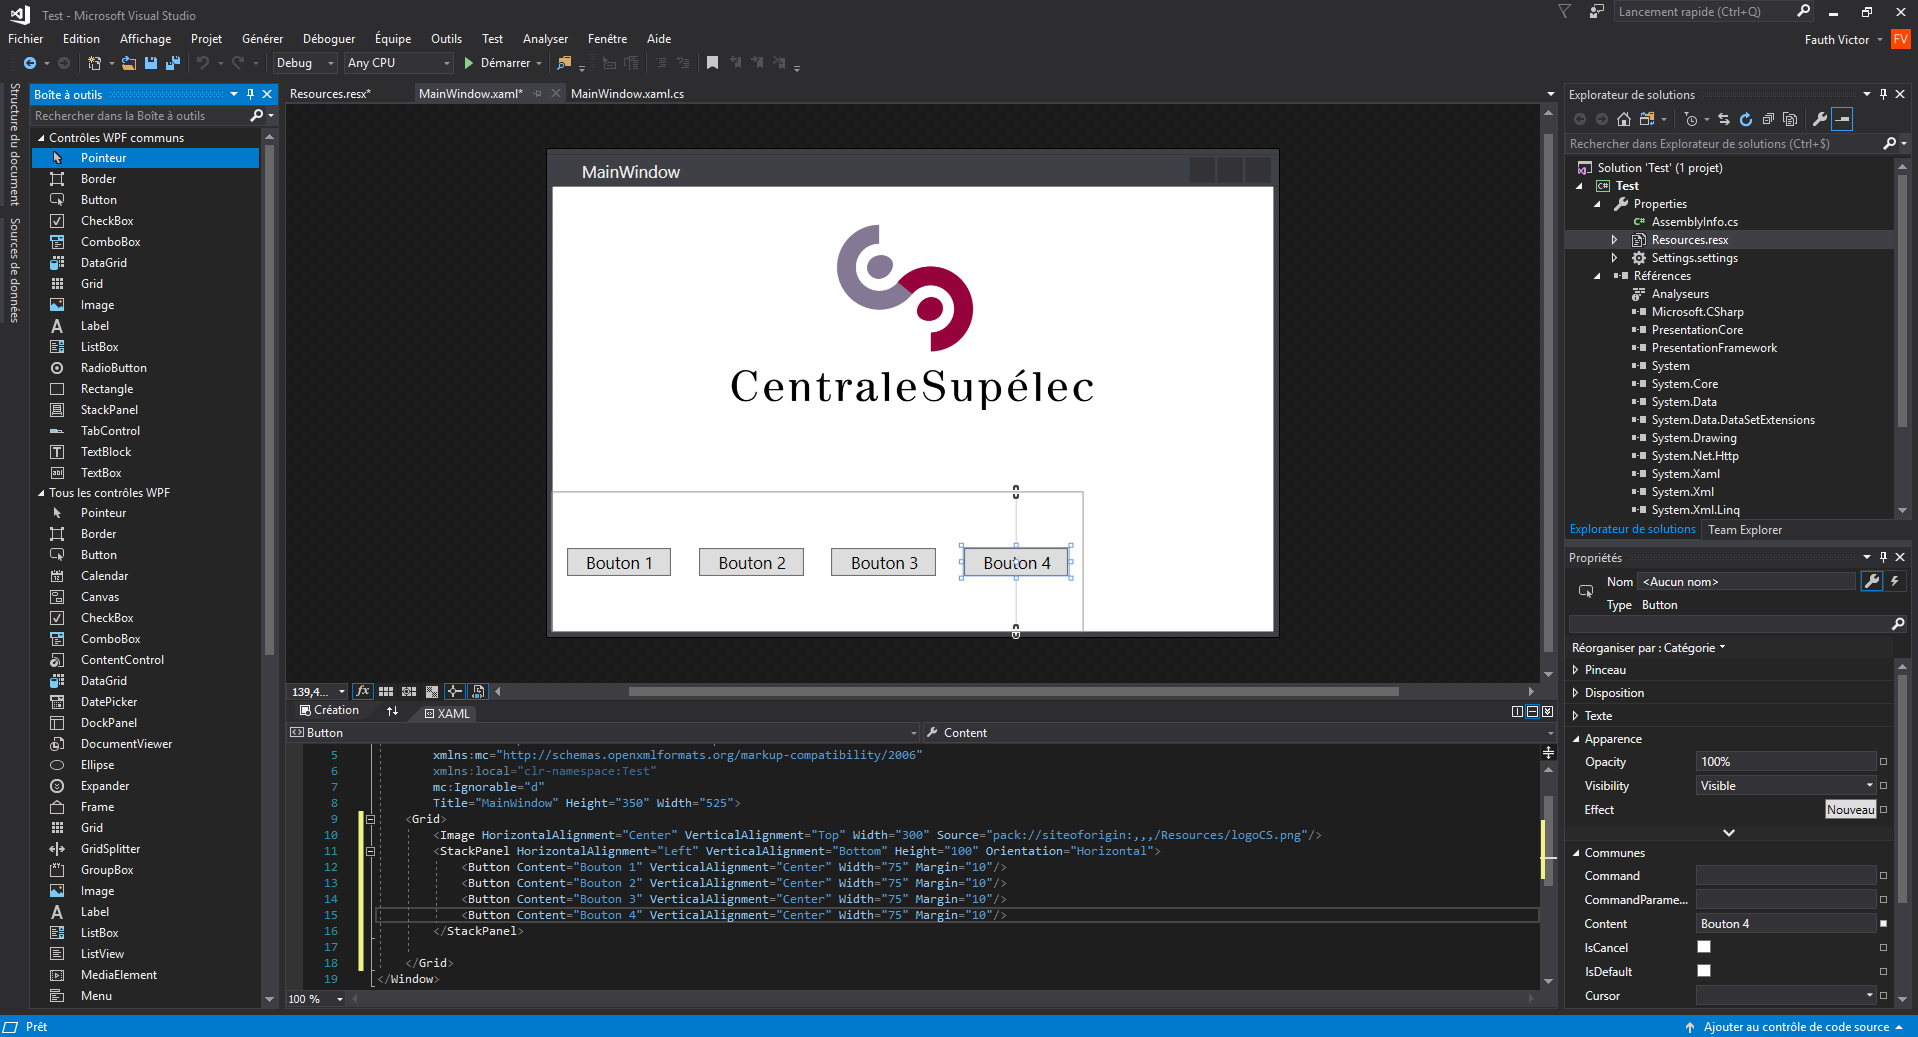
\includegraphics[width=1\textwidth]{editorXAML.png}
	\caption{L'éditeur graphique de XAML. Ici, une fenêtre avec une image et une ligne de boutons a été créée grâce à l'outil graphique, le code XAML correspondant est affiché dans la fenêtre inférieure. La fenêtre de droite permet de modifier les propriétés de l'élément sélectionné.}
	\label{fig:editorXAML}
\end{figure}


\section{Règles du jeu}

\paragraph{}Il s'agit d'un jeu très simple dans lequel un certain nombre de cartes sont posées, face cachée. Ces cartes vont par paire : chaque motif est représenté sur deux cartes. Les cartes sont posées au hasard, puis le joueur retourne deux cartes. Si elles sont identiques, la paire est retirée du jeu. Sinon, elles sont retournées face cachée, au même endroit (après un temps, ici deux secondes, permettant au joueur de mémoriser les cartes). Le jeu s'arrête lorsque toutes les paires ont été trouvées, le but étant de minimiser le nombre d'essais.


\section{Implémentation}

\subsection{Le modèle MVC}

\paragraph{}Pour coder le jeu, nous avons décidé d'utiliser l'architecture MVC (Modèle-Vue-Contrôleur). Le principe est de séparer le code en trois composantes distinctes : le modèle contient les données du programme, le contrôleur gère la logique et la vue interagit avec l'utilisateur.

\begin{figure}[H]
	\centering
	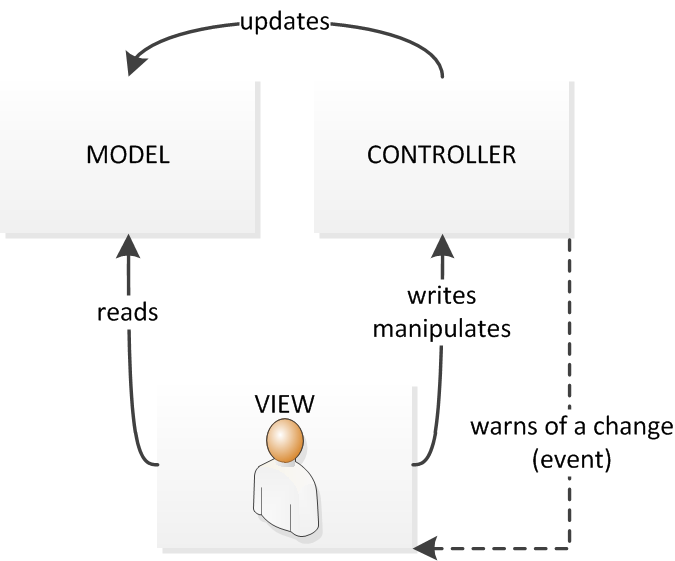
\includegraphics[width=1\textwidth]{modeleMVC.png}
	\caption{Les interactions de l'architecture MVC. Image tirée de Wikipédia.}
	\label{fig:MVC}
\end{figure}

\paragraph{\textbf{Remarque}} La structure de chaque classe est donnée en \autoref{sec:memory_annexe}.
\subsubsection{Le modèle}

\paragraph{}Le modèle contient l'état du jeu a un moment donné. Pour cela, nous définissons deux classes : la classe \lstinline|Card| et la classe \lstinline|Board|. \lstinline|Card| représente une carte et définit son état (trouvée et/ou affichée) ainsi que la pair dont fait partie la carte, tandis que \lstinline|Board| représente tout le plateau de jeu et contient notamment toutes les cartes, ainsi que le compteur de tours pour la partie en cours. Il possède une méthode pour incrémenter ce compteur, appelée à chaque fois que le joueur a désigné deux cartes, et deux méthodes utilisées lors de l'initialisation du plateau de jeu.


\subsection{Le contrôleur}

\paragraph{}Le contrôleur a la responsabilité de toute la logique du jeu. Il possède peu d'attributs, le stockage des données étant du ressort du modèle : deux attributs servent juste à référencer la vue et le plateau de jeu, le troisième enregistre quelle carte a été choisie par le joueur en attendant qu'il en choisisse une seconde. 

\paragraph{}Il y a cependant bien plus de méthodes, qui sont appelées lorsque le joueur agit. La méthode \lstinline|CardChosen| est appelée lorsque le joueur choisit une carte. S'il en a déjà choisi une juste avant, cette méthode vérifie si les deux cartes forment une paire avec \lstinline|CheckPair|, puis agit en conséquence. La méthode \lstinline|NextTurn| est alors appelée, et prépare le tour suivant, notamment en cachant à nouveau les cartes choisies précédemment (si elles ne constituaient pas une paire). C'est aussi elle qui va gérer la fin du jeu avec les méthodes \lstinline|IsFinished| (qui renvoie une booléen indiquant si toutes les paires ont été trouvées ou non ) et \lstinline|Exit| qui demande à la vue d'afficher la fenêtre de fin de partie.

\subsection{La vue}

\subsubsection{L'interface graphique statique en XAML}

\paragraph{}Le jeu gère n'importe quel nombre (pair) de cartes, nous n'avons donc pas défini l'interface graphique de manière statique en XAML : la classe \lstinline|Display| se charge de créer la totalité de l'affichage et de charger les images présentes dans le dossier pour les afficher en fonction du nombre de cartes souhaité. Le code XAML est donc presque vide, seule un élément \lstinline|Grid| est défini. Celui-ci s'étend sur l'intégralité de la surface de la fenêtre et permet juste de positionner facilement les cartes.


\subsubsection{L'interactivité en C\#}

\paragraph{}La classe \lstinline|Display| contient donc toutes les méthodes pour charger les images, créer les cartes à partir de ces images et des données du modèle, afficher et rafraîchir le plateau de jeu, et afficher la fenêtre des scores en fin de partie. Il s'agit de la classe la plus complexe à coder : pas à cause de sa logique, mais parce que cela a nécessite de bien comprendre le fonctionnement de WPF. Si le contrôleur et le modèle furent assez simple à coder, c'est parce qu'il s'agissait de programmation \enquote{générique}, à laquelle nous sommes déjà habitués, et le C\# n'est pas un langage extrêmement complexe à prendre en main si nous sommes déjà habitués au C++ ou au Java. Cependant, le WPF est extrêmement particulier, et, bien qu'il soit extrêmement puissant, de nombreux concepts sont difficiles à prendre en main et nécessitent de se plonger dans la documentation. Cela fut très instructif, nécessaire pour la suite du projet, et surtout formateur. 


\begin{figure}[H]
	\centering
	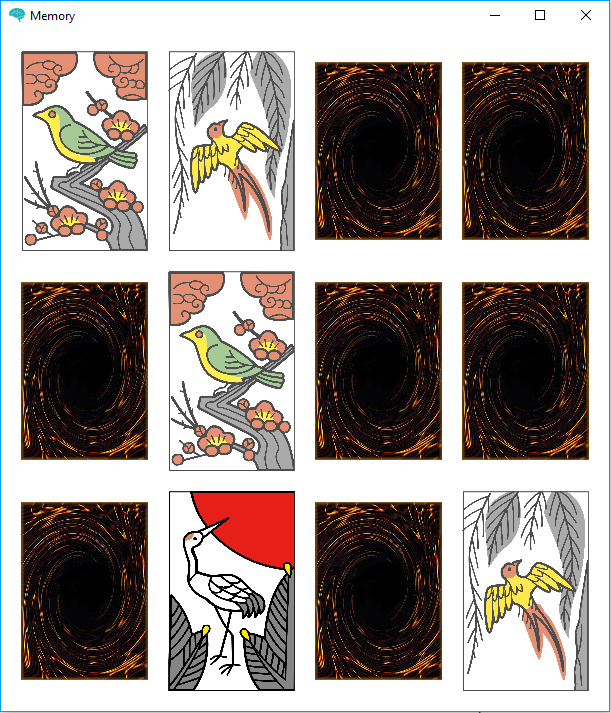
\includegraphics[width=1\textwidth]{memory.png}
	\caption{Une partie avec 16 cartes. Deux paires ont été trouvées, et une carte a été sélectionnée.}
	\label{fig:memory}
\end{figure}

\newpage
\subsection{Annexe}
\label{sec:memory_annexe}

\lstinputlisting[caption=La structure de la classe \lstinline|Card| du modèle.]{Sources/Model/Card.cs}
\newpage
\lstinputlisting[caption=La structure de la classe \lstinline|Board| du modèle.]{Sources/Model/Board.cs}
\newpage
\lstinputlisting[caption=La structure de la classe \lstinline|Game| du contrôleur.]{Sources/Controller/Game.cs}
\newpage
\lstinputlisting[caption=La structure de la classe \lstinline|Display| de la vue.]{Sources/View/Display.cs}
